
\section{Methodology}
\label{sec:methods}


\def\ue{\ensuremath{\vec{\tilde{u}}\earth}}


The essential approach of motion correction is to measure velocity on a moving platform and make an independent measurement of the platform motion, then subtract the motion from the velocity measurements. This approach has been used to successfully correct sonic anemometer measurements of atmospheric turbulence \cite[e.g., ][]{Edson++1998, Miller++2008}.  In the ocean, previous works have utilized inertial motion sensors to quantify the motion of multiscale profilers for the purpose of measuring the full spectrum of oceanic shear \cite[]{Winkel++1996}.

Nortek's ADV-IMU measures the linear acceleration, $\Accel$, rotational motion, $\AngRt$, and orientation matrix, $\omat$, of the ADV pressure case (body) in the Earth reference frame. The Microstrain IMU integrated into the Nortek Vector ADV has been configured to provide estimates of the ADV's orientation and motion at every time step of the ADV's sampling (the time synchronization is $O(10^{-2}\ \mathrm{s})$). So long as the ADV head is rigidly connected to the IMU (ADV pressure case), the motion of the ADV head is calculated from these signals as the sum of rotational and translational motion:
\begin{align}
  \label{eqn:uhead}
\begin{split}
  \uhead & = \urot + \uacc + \ulow \\
      & = \omatinv \cdot \AngRt^*(t)\times\l + \int \{\Accel(t)\}_{HP(f_{a})} \mathrm{d}t + \ulow
\end{split}
\end{align}
Here, $*$ superscripts denote quantities in the ADV's local coordinate system, and $\l$ is the vector from the IMU to the ADV head. $\omatinv$---the inverse of the orientation matrix---rotates vectors from the IMU to the Earth reference frame. The notation $\{\Accel\}_{HP(f_a)}$ indicates that the IMU's accelerometer signal is high-pass filtered (in the Earth's stationary reference frame) at a chosen filter frequency, $f_a$. Without such filtering, low-frequency noise in $\Accel$---sometimes referred to as bias drift---is amplified by integration to the point that it overwhelms the higher frequency information \cite[]{Barshan+Whyte1995, Bevly2004, Gulmammadov2009}.

\begin{figure}
  \centering
  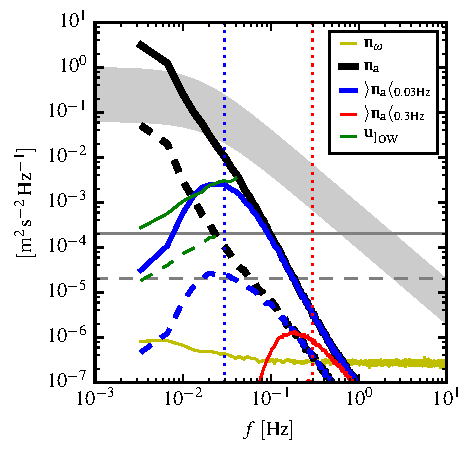
\includegraphics[width=\onewidth]{stationary_noise04}
  \caption{Spectra of $\urot$ (yellow) and $\uacc$ signals from the Microstrain IMU sitting on a motionless table. The $\uacc$ signals are unfiltered (black), and high-pass filtered at 30 s (magenta) and 5 s (green). Vertical dotted lines indicate the filter frequency.  Blue lines are an estimate of $\ulow$ for the TTM. Solid lines are the horizontal components, and dashed lines are the vertical components of $\uacc$ and $\ulow$. The horizontal and vertical Doppler noise levels of a Nortek Vector ADV configured to measure $\pm$4m/s are indicated by horizontal dash-dot and dotted lines, respectively. The shaded region indicates the range of $u$ spectral amplitudes presented herein (0.002 $< \tke <$ 0.03 $\mathrm{m^2/s^2}$, 1e-5 $< \epsilon <$ 5e-4 $\mathrm{W/kg}$).}
  \label{fig:stnoise}
\end{figure}

The spectra of $\uacc$ and $\urot$ from an ADV-IMU resting motionless on a table are instructive in understanding the importance of filtering (Figure \ref{fig:stnoise}). Because the IMU is stationary, these spectra indicate the noise levels of each signal.  The noise level of $\spec{\urot}$ (yellow) is several orders of magnitude lower than the velocity spectra we measured (grey region), and also more than an order of magnitude smaller than the Doppler noise levels of the ADV. Here we have used $\l=1$ m; which is the order-of-magnitude of the typical distance between the ADV head and the IMU. This indicates that the precision of $\urot$ (i.e. the angular rate sensor) is adequate for making corrections to ADV velocity measurements without filtering.

The noise level of $\spec{\uacc}$ (Figure \ref{fig:stnoise}, black), on the other hand, is dominated by a $f^{-2}$ slope that results from integrating the low-frequency noise in $\Accel$. The high-pass filtering reduces this noise so that it does not contaminate motion correction, but real motion at these frequencies is lost \cite[]{EgelandPhD2014, VanZwieten++2015}. This means that there is a residual low-frequency translational motion, $\ulow$, that needs to be measured independently---or at the very least considered---when using motion-corrected ADV-IMU data. 

The choice of a high-pass filter for reducing low-frequency accelerometer noise depends on the application of the measurement and the platform being used. In particular, filter selection involves a trade-off between filtering out the bias drift noise while not filtering out measured motion that is unresolved by an independent measurement of $\ulow$. Note that, to avoid double counting, $\ulow$ should be estimated by applying the complementary low-pass filter to the independent measurement of low-frequency motion. We use 4$^\mathrm{th}$-order, bidirectional (zero-phase), Hanning filters for all filtering operations. 

For the StableMoor buoy, the ADP bottom-track agrees with $\uacc$ over a narrow frequency band (see appendix \ref{apdx:ulow}), indicating that the ADP and IMU are resolving the same motion. Furthermore, $\ulow$ derived from the ADP bottom-track gives a noteworthy improvement in the shape of $\spec{u}$ and $\spec{v}$ when compared to similar spectra that assume $\ulow=0$. In the latter case, spectral peaks and dips are present between 0.01 and 0.1 Hz that are inconsistent with other measurements of oceanic turbulence (not shown). This indicates that ADP bottom-track measurements are important for resolving turbulence spectra from the StableMoor buoy platform. For the StableMoor buoy we utilize $f_a = 0.2 Hz$ (5-s period); further details of this choice can be found in appendix \ref{apdx:ulow}.
%in these   component of motion correction of  is because the StableMoor motion is at a lower frequency where the IMU accelerometers perform poorly (motion contamination is persistent if we assume $\ulow=0$), and because the ADP probably provides a more accurate estimate of $\ulow$ than the rigid pole model does for the TTM. 

For the TTM the ADV position, relative to its base, can be estimated by assuming the mooring acts like a rigid pole and using the IMU orientation matrix to estimate the pole's `lean'. The position obtained from this model can then be differentiated to estimate $\ulow$. Because the mooring is not actually a rigid pole this approach is likely to over-estimate $\ulow$, particularly at high frequencies where wobbling and swaying deviate from the rigid-pole model. At low-frequencies, we believe this approach provides a reasonable estimate of maximum head motion.

Spectra of $\ulow$ estimated using this approach for the June 2014 TTM deployment (Figure \ref{fig:stnoise}, blue) are plotted up to the point where they cross their respective $\spec{\uacc}$ noise level (black); beyond this frequency we assume $\spec{\uacc}$ provides a better estimate of the translational motion noise-level then the rigid pole model.  Together, these two lines provide an `aggregate noise level' of translational velocity estimates from the TTM: the rigid pole estimate of $\ulow$ indicates the amplitude of unresolved motion at low-$f$ (blue), and $\spec{\uacc}$ indicates the limits of the IMU at high-$f$ (black). Coincidentally, $\spec{\uacc}$ filtered at $f_a = 0.0333$Hz is not a terrible approximation for this aggregate noise level. We did use an estimate of $\ulow$ based on this model, but---because the aggregate noise level is at least 10$\times$ lower than the velocity spectra of interest (shaded region)---those results were equivalent to assuming that $\ulow = 0$ and using $f_a = 0.0333$Hz (30-s period). Thus, we simply used $\ulow=0$ and $f_a=0.0333$Hz for the TTM and the turbulence torpedo estimates of $\uhead$.

With this estimate of ADV head motion, it is straightforward to correct the measured velocity, $\umeas$, to estimate the velocity in the Earth's inertial reference frame:
\begin{align}
  \label{eqn:u_mot_def}
  \ue(t) & = \umeas(t) + \uhead(t).
\end{align}
Note here that the `+'-sign is correct because head motion, $\uhead$, induces a measured velocity in the opposite direction of the head motion itself ($\umeas = \ue - \uhead$).

Additional details on motion correction---including a detailed accounting of the distinct coordinate systems of the IMU, ADV pressure case, and ADV head---can be found in \cite{Kilcher++2016}. Open-source Python tools for performing motion correction of ADV-IMU data---including scripts that write processed data in Matlab and tabulated formats---are available at \url{http://lkilcher.github.io/dolfyn/}.

\def\ue{\ensuremath{\vec{u}\earth}}

%%% Local Variables:
%%% mode: latex
%%% TeX-master: "Kilcher_etal_IMU-ADV"
%%% End:
